\documentclass{beamer}
\usepackage{animate}
\usepackage{multimedia}
\usepackage[english,russian]{babel}

\usepackage{pgfpages}
\setbeameroption{show notes on second screen}
%https://tug.ctan.org/macros/latex/contrib/beamer/doc/beameruserguide.pdf

\usepackage[T2A]{fontenc}
\usepackage[utf8]{inputenc}

\setbeamertemplate{caption}[numbered]

\usetheme{CambridgeUS}
\usecolortheme{dolphin}


\title[Введение в КГ]{Введение в компьютерную графику}
\author[Быковских Д.А.]{Быковских Дмитрий Александрович}
\date{02.09.2023}

\begin{document}
	\begin{frame}
		\titlepage
	\end{frame}
	%\section{Обзор}
	\begin{frame}{Содержание}
		\begin{itemize}
			\item 
			Общая информация о компьютерной графике
			\item
			Некоторые факты из истории компьютерной графики
			\item
			Аппаратные средства, связанные с выводом изображения
			\item 
			Библиотеки визуализации
		\end{itemize}
	\end{frame}
	\begin{frame}{Что такое компьютерная графика?}
		Компьютерная графика --- одно из направлений информационных технологий, которое занимается созданием, редактированием и визуализацией \textbf{графических изображений}.
		
		Спектр применений:
		
		\begin{columns}
			
			\begin{column}{0.5\textwidth}
				\begin{itemize}
				\item
				Разработка игр (виртуальный мир, персонажи, эффекты)
				
				\item
				Визуализация данных (диаграммы, графики)
				\item
				Дизайн (логотипы, баннеры, упаковки, интерфейсы)
				\item
				Симуляция и моделирование (создание виртуальных сред для тестирования и исследования различных сценариев)
				
			\end{itemize}
			\end{column}
			\begin{column}{0.5\textwidth}
				\begin{itemize}
				\item
				Анимация (фильмы, видеоролики, реклама)
				\item
				Медицинская визуализация (модели органов, тканей и других частей тела, )
				\item
				Архитектурное проектирование (модели жилых районов, зданий, интерьеров)
				\item
				Редактирование фотографий и видеороликов (улучшение качества изображений)
			\end{itemize}
			\end{column}
		
		\end{columns}
		
		
		\if 0
		3D-моделирование и анимация: Создание трехмерных моделей объектов, персонажей и сцен, а также их анимация для использования в фильмах, играх, визуализации архитектурных проектов и многих других областях.
		
		2D-графика и иллюстрации: Создание двумерных изображений, иллюстраций, рисунков, артов и графических элементов для книг, журналов, рекламы и дизайна.
		
		Визуализация данных: Преобразование сложных данных в наглядные и понятные визуальные формы, такие как графики, диаграммы, инфографика и карты.
		
		Компьютерная анимация и эффекты: Создание анимаций, спецэффектов и визуальных элементов для фильмов, рекламы, игр и других медийных продуктов.
		
		Графический дизайн: Разработка дизайна логотипов, брендинга, упаковки, веб-сайтов, приложений и других визуальных элементов.
		
		Виртуальная реальность (VR) и дополненная реальность (AR): Создание виртуальных и дополненных миров, в которых пользователи могут взаимодействовать и иметь визуальный опыт.
		
		Компьютерное моделирование: Создание компьютерных моделей и симуляций для изучения поведения систем, процессов и явлений в науке, инженерии и других областях.
		
		Медицинская визуализация: Создание графических изображений и моделей для обучения, диагностики и планирования медицинских процедур.
		
		Архитектурная визуализация: Создание виртуальных моделей зданий и помещений для архитекторов и дизайнеров.
		
		Ретушь и обработка фотографий: Использование графических инструментов для улучшения и изменения фотографий.
		
		Генеративное искусство: Использование алгоритмов и программирования для создания уникальных искусственных изображений и анимаций.
		\fi
		
	\end{frame}
	
	\begin{frame}
		
		\centering
		\textbf{Основные направления}
		
		\begin{columns}
			\begin{column}{0.3\textwidth}
				
				Computer Vision
				
				Machine Learning
				
				Data Mining
				\begin{figure}
				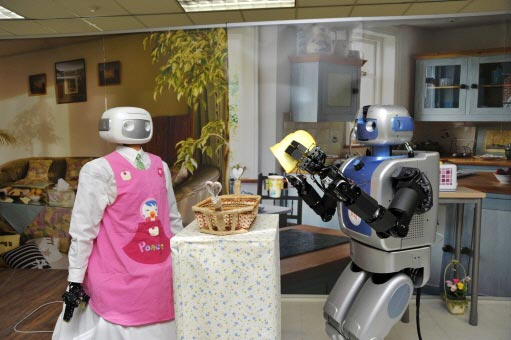
\includegraphics[width=\textwidth]{images/Computer_vision.png}
				\caption{Семейная пара}
				\end{figure}
			\end{column}
			
			\begin{column}{0.4\textwidth}
				
				Computer Graphics
				
				Computer-Generated Imagery
				
				Realtime Processing
				\begin{figure}
				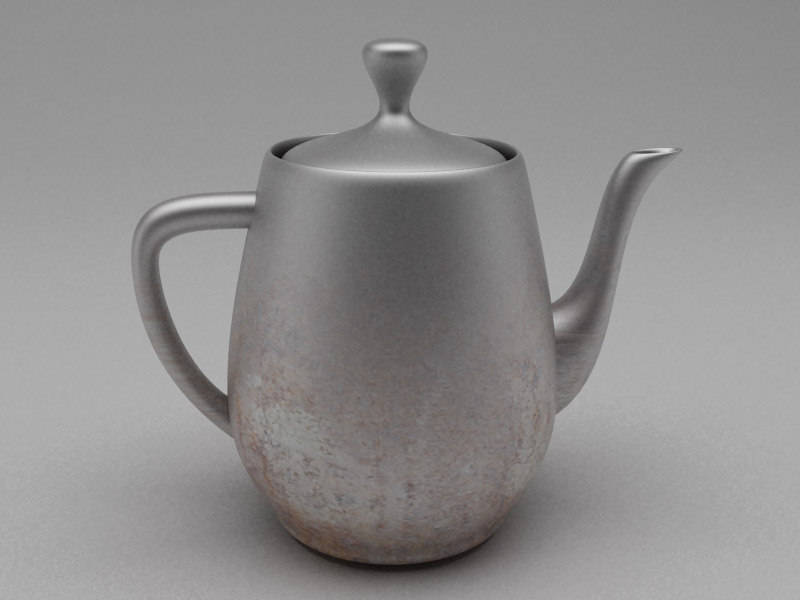
\includegraphics[width=\textwidth]{images/Utah_teapot.png}
				\caption{Чайник Юта}
				\end{figure}
				
			\end{column}
			
			\begin{column}{0.3\textwidth}
				
				Image Processing
				
				Image Compression
				
				Noise Reduction
				\begin{figure}
				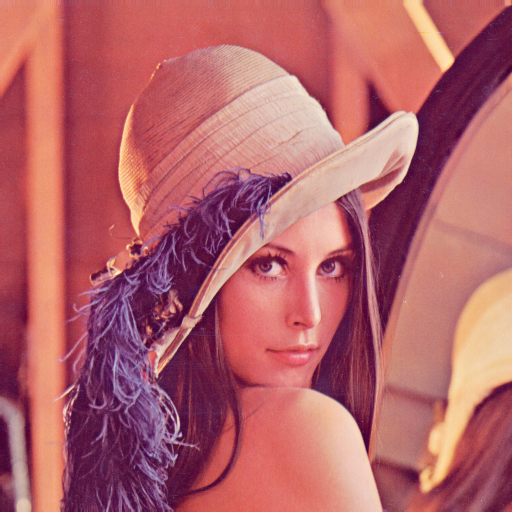
\includegraphics[width=\textwidth]{images/Lenna_test_image.png}
				\caption{Лена Сёдерберг}
				\end{figure}
				
			\end{column}
		\end{columns}
	\end{frame}
\if 0	
	\begin{frame}
	%https://iasl.uni-muenchen.de/links/GCA-IV.2e.html
	%https://www.timetoast.com/timelines/6248910a-e70f-4a32-b27c-e13ef9c355dc
	%https://web.archive.org/web/20070405181508/http://accad.osu.edu/\%7Ewaynec/history/lesson2.html
	%https://web.archive.org/web/20051103164835/http://accad.osu.edu/~waynec/history/lesson2.html
	

	История компьютерной графики насчитывает несколько десятилетий и прошла через ряд важных этапов и достижений. Вот краткий обзор этой истории:
	
	1950-е годы: Ранние исследования в области компьютерной графики начались в 1950-х годах. В 1950 году Иван Сазерленд (Ivan Sutherland) создал устройство "Скетчпад" (Sketchpad), позволяющее рисовать графику с помощью светового пера и дисплея.
	
	1960-е годы: В 1963 году Сазерленд представил прототип первого компьютерного графического устройства для рисования 3D-изображений, названного "TX-2 Sketchpad". Этот момент считается началом трехмерной компьютерной графики.
	
	1970-е годы: В 1970-х годах были разработаны первые программы для создания и редактирования графики, такие как "SuperPaint" и "Computer Graphics System" на основе аппаратных решений. Были также созданы первые алгоритмы заполнения и отсечения для растровой графики.
	
	1980-е годы: В это десятилетие произошли значительные прорывы в компьютерной графике. Были разработаны первые графические интерфейсы пользователя (GUI), например, интерфейс для компьютера Apple Macintosh. Также были созданы первые 3D-моделирование и анимационные программы.
	
	1990-е годы: С распространением персональных компьютеров и улучшением аппаратного обеспечения появились новые возможности для компьютерной графики. Были разработаны 3D-игры, программы для редактирования фотографий и видеороликов.
	
	2000-е годы: Развитие 3D-графики продолжилось, и стали доступны более мощные инструменты для создания сложных 3D-моделей и анимаций. Также стали популярными виртуальная и дополненная реальность.
	
	2010-е годы: Продолжалось усовершенствование компьютерной графики, включая разработку более реалистичных графических движков для видеоигр, прорывы в области визуализации данных и рост популярности анимации и цифрового искусства.
	
	\end{frame}
\fi
	
	\section{История развития. Интересные факты}
	
	\begin{frame}{Одна из первых компьютерных игр --- Spacewar}{1962 г.}
	
	\begin{columns}
		
		\begin{column}{0.5\textwidth}
			
			%Название: Spacewar!
			
			Жанр: Shoot’em up, космический симулятор
			
			Авторы: Steve Russell, Martin Graetz, Wayne Wiitanen, Bob Saunders, Steve Piner
			
			%Платформа: DEC PDP-1
			
			Длительность разработки: 200 Чч
			
		\end{column}
		\begin{column}{0.5\textwidth}
			\begin{figure} 
			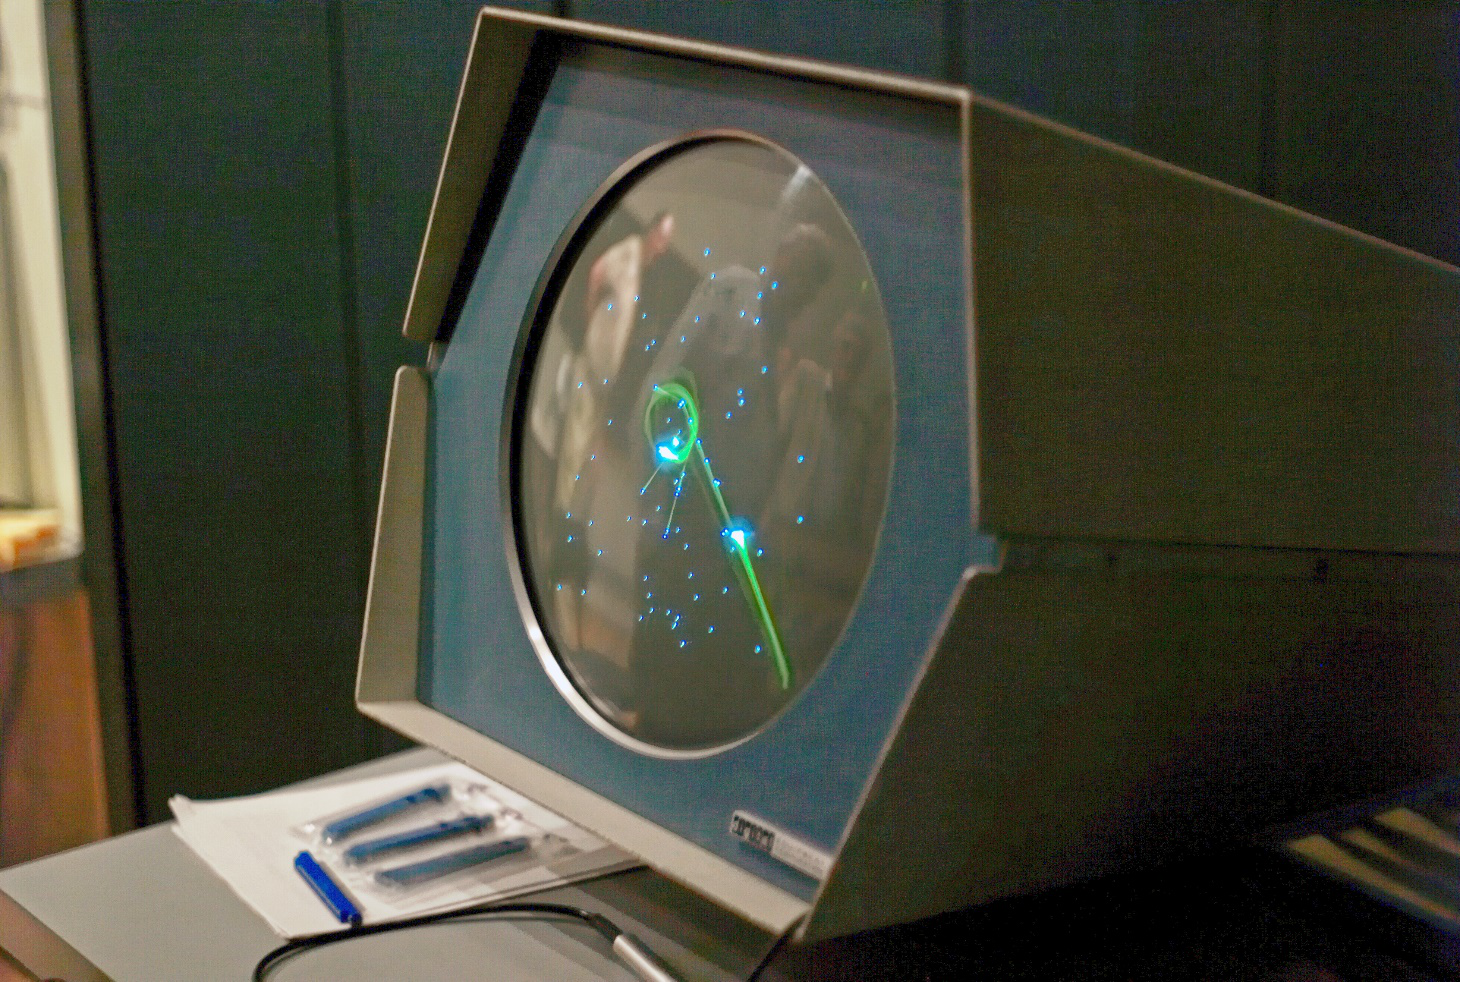
\includegraphics[width=\textwidth]{images/Spacewar.png}
			\caption {DEC PDP-1 and Spacewar}
			\end{figure}
		\end{column}
		
	\end{columns}
	
	
	\end{frame}

\begin{frame}{Одна из первых компьютерных анимаций}
	{1968 г.}
	
	\begin{columns}
		\begin{column}{0.5\textwidth}
			
			Название: Кошечка
			
			Авторы: Н.Н. Константинов, В. Минахин, В. Понаморенко, А. Скуридин, В. Журкин
			
			Платформа: БЭСМ-4 и алфавитно-цифровой принтер
			
			Реализация: движение кошки описаны дифференциальными уравнениями
			
		\end{column}
		\begin{column}{0.5\textwidth}
			\begin{figure}
				\href{https://www.youtube.com/watch?v=LzMk5sC6eAU}{
				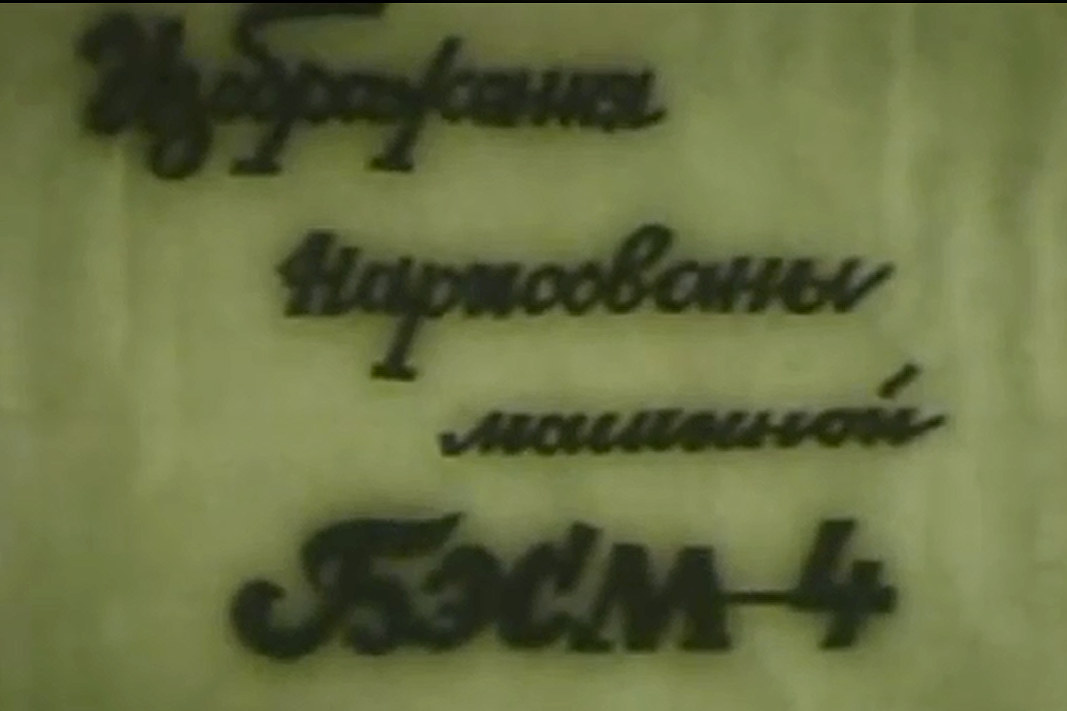
\includegraphics[width=\textwidth]{images/AnimatedCat.jpg}
				}
				\caption {Кошечка}
			\end{figure}
		\end{column}
	\end{columns}
\end{frame}

\begin{frame}{Чайник Юта (Newell teapot)}{1975 г.}
	\begin{columns}
		\begin{column}{0.5\textwidth}
			\begin{figure} 
				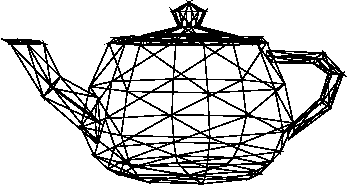
\includegraphics[width=\textwidth]{images/Utah_teapot_model.png}
				\caption {Состоит из 32-хкубических поверхностей Безье}
			\end{figure}
		\end{column}
		\begin{column}{0.5\textwidth}
			\begin{figure} 
				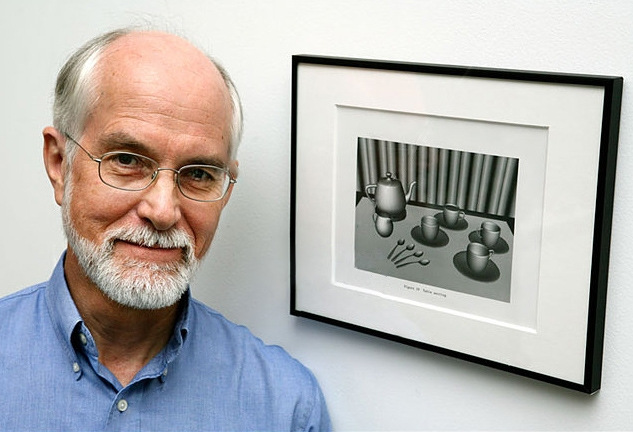
\includegraphics[width=\textwidth]{images/Utah_teapot_and_Newell.png}
				\caption {Мартин Ньювелл и чайник Юта}
			\end{figure}
		\end{column}
	\end{columns}

	\note{
		https://www.opengl.org/resources/libraries/glut/spec3/node89.html
		
		Скомпилировать программу из 
		CG/Projects/src/utah\_teapot.c
	}

\end{frame}

\begin{frame}{Silicon Graphics Inc. (SGI)}{1982 г.}
	\begin{columns}
		\begin{column}{0.5\textwidth}
			
			Описание: Разработка графических станций (Indigo, Indy и др.) и ПО (SGI IRIX и др.) для визуализации
			
			Основатель: Джим Кларк
			
		\end{column}
		\begin{column}{0.5\textwidth}
			\begin{figure} 
				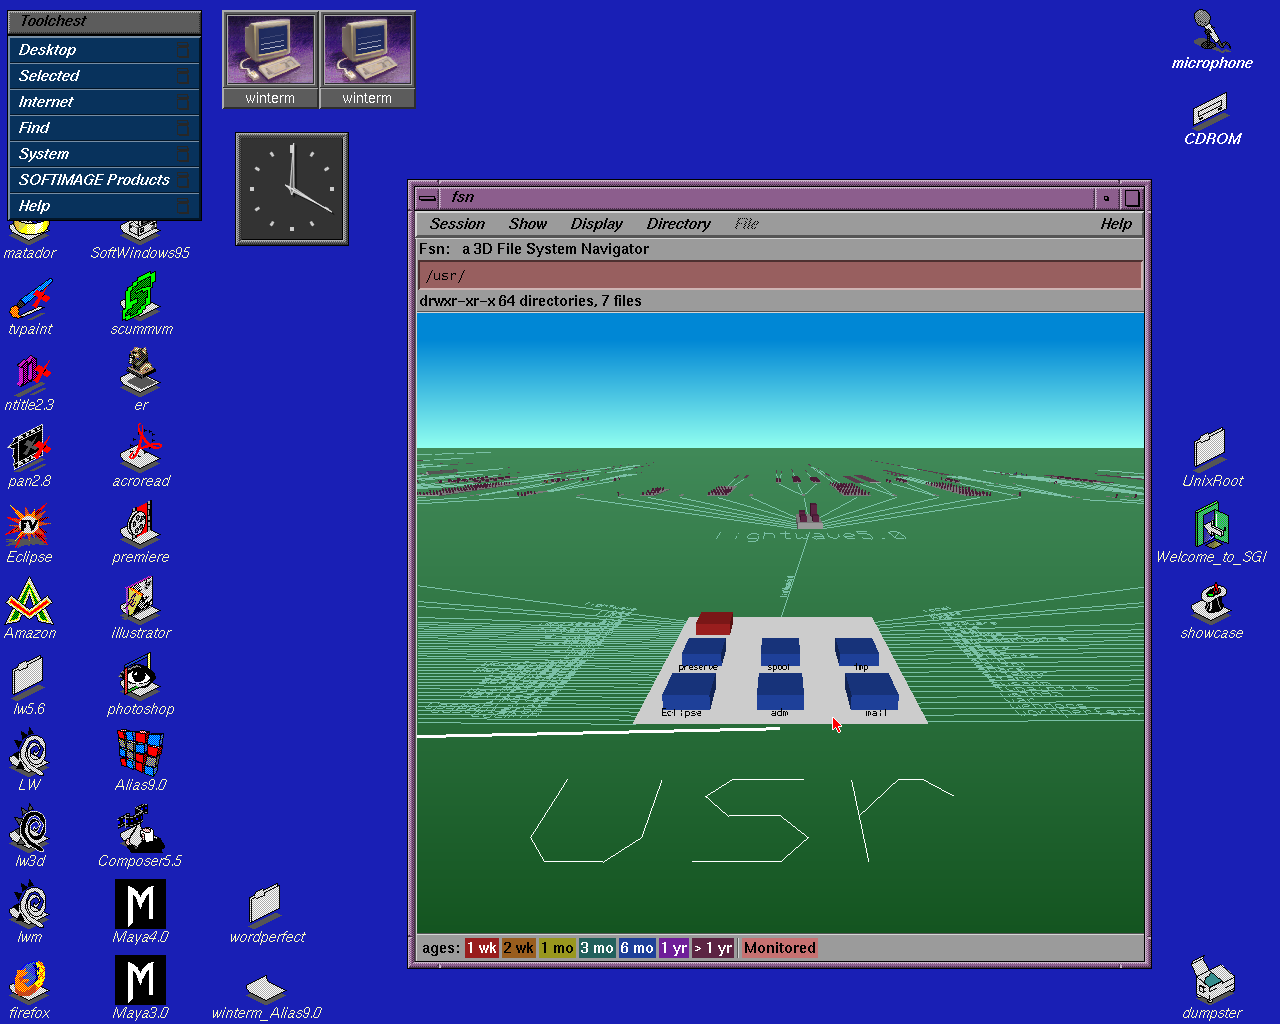
\includegraphics[width=\textwidth]{images/IRIX_OS.png}
				\caption {IRIX OS}
			\end{figure}
		\end{column}
	\end{columns}
	\note{
		История компании Silicon Graphics

	https://habr.com/ru/companies/vdsina/articles/562912/	

	{
	\scriptsize

		В 1984 году SGI выпустила системы IRIS первого поколения (модели 1000 и 1200).

		Вскоре получила статус легенды среди 3D-художников и графических дизайнеров, использовавших уникальную мощь её рабочих станций.

		Наследие можно увидеть в Nintendo 64 (вышла в 1996 г.). 
		
		Принимала участие в разработке голливудских фильмов, включая 
		Jurassic Park, «Парк юрского периода» (1993 г.),
		Jumanji, «Джуманджи» (1995 г.),
		The Matrix, «Матрица» (1999 г.),
		Star Wars. Episode I, «Звёздные войны. Эпизод I» (1999 г.),
		Lord of the Rings, «Властелин колец» (2000 г.),
		и другие.

		В 1992 году SGI решили перепроектировать API и начали продавать недорогие лицензии на него своим конкурентам.
		После SGI организовала OpenGL Architecture Review Board для руководства дальнейшими разработками.

		В феврале 1996 года SGI решила войти на рынок суперкомпьютеров, приобретя за 740 миллионов долларов Cray Research.

		В 2003 году компания освободила помещения своей штаб-квартиры в Маунти-Вью и сдала здание в аренду Google.

		В апреле 2009 года снова SGI подала заявку согласно Главе 11 и была продана Rackable Systems за 25 миллионов.
		
		\_
		
		}
	}

\end{frame}


\begin{frame}{Первая 3D видеокарта}{1996 г.}
	\begin{columns}
		\begin{column}{0.5\textwidth}
			
			\begin{figure}
				\href{https://www.youtube.com/watch?app=desktop&v=Zdf270cZD9g}{
				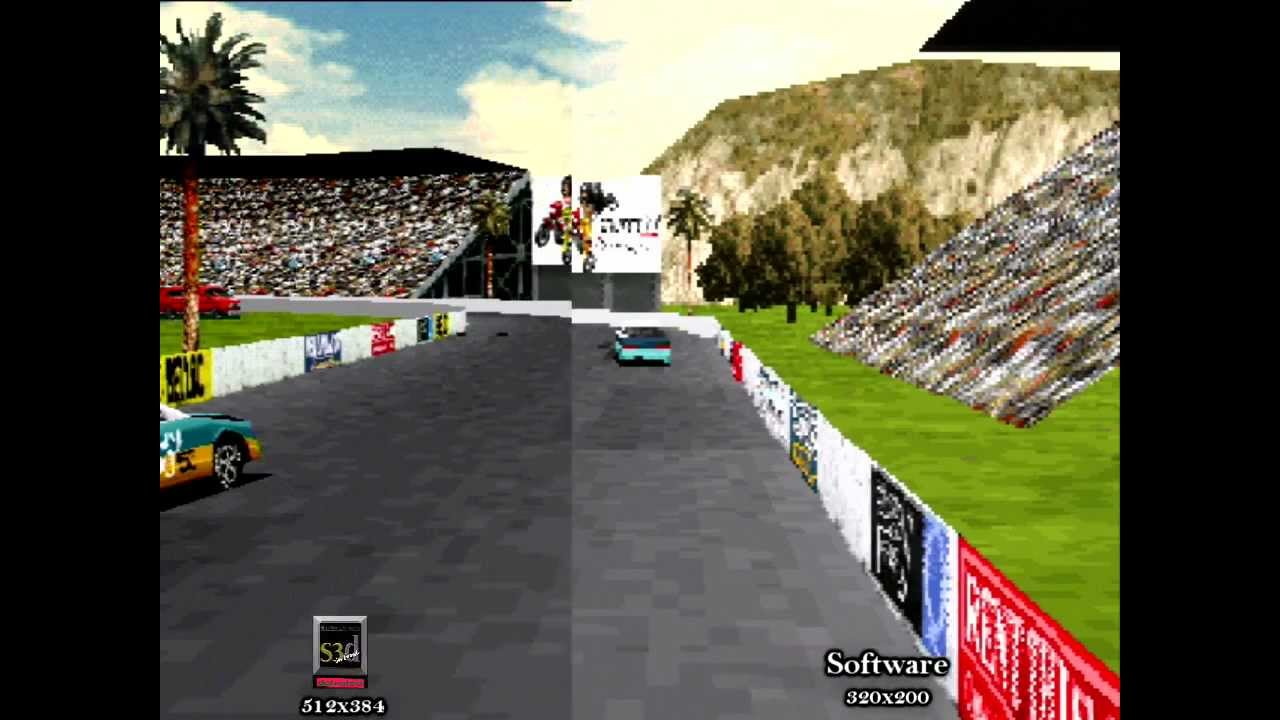
\includegraphics[width=\textwidth]{images/Destruction_Derby_1995.png}}
				\caption {Destruction Derby (1995 г.)}
			\end{figure}
		\end{column}
		\begin{column}{0.5\textwidth}
			\begin{figure} 
				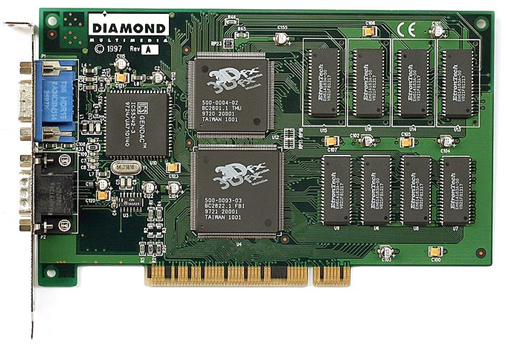
\includegraphics[width=\textwidth]{images/Diamond_Monster_3D_3DFX_Voodoo1.png}
				\caption {Diamond Monster 3DFX Voodoo1}
			\end{figure}
		\end{column}
	\end{columns}
\end{frame}

\section{Аппаратные средства}

\begin{frame}{Характериситки видеокарты 3DFX Voodoo1}{1996 г.}
	\begin{columns}
		\begin{column}{0.5\textwidth}
			Разработчик: Diamond
			
			Шины I/O: PCI/VGA
			
			Память: 4 MB EDO DRAM
			
			Тех процесс: 500 nm
			
			Частота min/max: 45/50 MHz
			
			DirectX: DX5
			
			Цена: 300\$
			
			Эффекты: texture modulation, Z-buffering, Bi-linear texture filtering, anti-aliasing etc.
		\end{column}
		\begin{column}{0.5\textwidth}
			\begin{figure} 
				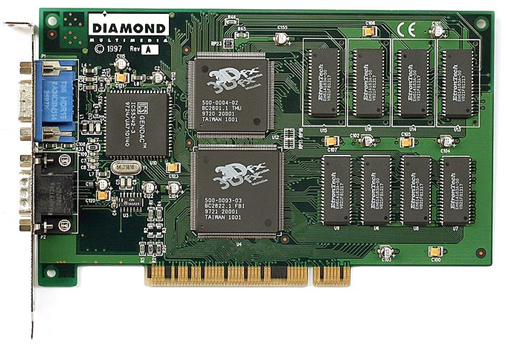
\includegraphics[width=\textwidth]{images/Diamond_Monster_3D_3DFX_Voodoo1.png}
				\caption {Diamond Monster 3DFX Voodoo1}
			\end{figure}
			
		\end{column}
	\end{columns}
\note{
{\tiny
	\begin{enumerate}
		\item	
	\textbf{Texture Modulation (текстурная модуляция)} \\
	- это техника в компьютерной графике, которая позволяет комбинировать две или более текстуры в одной точке на поверхности объекта. Это достигается путем умножения цветов пикселей из различных текстур и последующим объединением результатов. Это может использоваться для создания сложных визуальных эффектов, таких как освещение, тени и детализация.
	
	\item
	\textbf{Z-buffering (Буфер глубины)} \\
	- это метод решения проблемы видимости в трехмерной графике. Он использует буфер глубины (или Z-буфер), который хранит информацию о расстоянии от камеры до каждого пикселя на экране. Во время рендеринга сцены каждый новый пиксель сравнивается с содержимым Z-буфера. Если новый пиксель ближе к камере, его глубина записывается в Z-буфер, и цвет пикселя рендерится на экране. Это обеспечивает правильное наложение объектов в сцене и решает проблему перекрытия.
	
	\item
	\textbf{Bi-linear Texture Filtering (Билинейная фильтрация текстуры) } \\
	- это метод интерполяции цветов пикселей на текстуре для сглаживания артефактов, таких как лестничные эффекты или пиксельные артефакты, которые могут возникнуть при растягивании или сжатии текстур. Для каждого пикселя на экране берутся ближайшие четыре пикселя на текстуре, и их цвета интерполируются на основе расстояния до центра пикселя на экране. Это обеспечивает более плавное и реалистичное отображение текстур на объектах.
	\item
	\textbf{Anti-aliasing (Сглаживание краев)} \\
	- это техника, которая используется для смягчения ступенчатых краев (лестничных эффектов) на объектах или линиях в компьютерной графике. Она достигается путем усреднения цветов пикселей, находящихся на границе объекта, с окружающими пикселями. Это создает плавный переход цветов и уменьшает эффект "мерцания" на границах объектов при их движении или вращении.
\end{enumerate}
}
}
\end{frame}


\begin{frame}{Характериситки видеокарты}{Графический процессор (видеочип)}
	Число транзисторов, трлн.
	
	Техпроцесс, нм
	
	Тактовая частота, ГГц
	
	Количество шейдерных ядер (ALU, Arithmetic Logic Unit)
	
	Тензорные ядра (Tensor Cores)

	RT-ядра (Ray-Tracing Cores)

	Скорость заполнения (Fill Rate)
	\begin{itemize}
		\item 
		Пиксельная – число блоков растровых операций (Raster Operations Pipeline
	or Render Output Unit, ROPs)
		\item 
		Текстурная – количество блоков наложения текстур (Texture Mapping Unit,
		TMUs)
	\end{itemize}
	
	
	\note{
	
		Описание самой мощной игровой видекарты на 2022 г.

		https://www.techpowerup.com/gpu-specs/geforce-rtx-4090.c3889

		С различными характеристиками можно ознакомиться здесь

		https://www.thg.ru/graphic/graphic\_card\_faq\_ii/index.html
		
		\tiny
		{\small
		Скорость заполнения (Fill Rate)
		}
	
		C какой скоростью графический процессор может выдавать пиксели (например,triangle fill rate у старых видеокарт). 
		Выделяют два типа скорости заполнения: пиксельную (pixel fill rate, ${PFR = ROP \cdot Hz }$) и текстурную (texture fill rate).

		Текстурную скорость заполнения ATi и nVidia считают по-разному. nVidia считает, что скорость получается умножением числа пиксельных конвейеров на тактовую частоту. А ATi умножает число текстурных блоков на тактовую частоту. В принципе, оба способа корректны, поскольку nVidia использует по одному текстурному блоку на блок пиксельных шейдеров, т.е. по одному на пиксельный конвейер.

		{\small
		Блоки наложения текстур (Texture Mapping Unit, TMU)
		}

		Текстуры следует выбрать и отфильтровать. Эта работа выполняется блоками наложения текстур, которые работают совместно с блоками пиксельных и вершинных шейдеров. 
		Работа TMU заключается в применении текстурных операций над пикселями.

		{\small
		Блоки растровых операций (Raster Operator Unit, ROP)
		}

		Процессоры растровых операций отвечают за запись пиксельных данных в память. Скорость, с которой выполняется эта операция, является скоростью заполнения (fill rate). 
		Производительность (и число) ROP уже редко используется для оценки скорости видеокарты, т.к. перестала быть узким местом. 

		\_
	}
	
\end{frame}

\begin{frame}{Характериситки видеокарты}{Графическая память и прочие атрибуты}
	\begin{columns}
		\begin{column}{0.5\textwidth}
			\textbf{Графическая память}
			
			Разрядность шины, бит
			
			Тип микросхем (GDDR5X SDRAM)
			
			Тактовая частота, ГГц
			
			Объем, Tбайт
		\end{column}
		\begin{column}{0.5\textwidth}
			\textbf{Другие атрибуты}
			
			Размеры
			
			Тип охлаждения
			
			Шина I/O (PCIe)
			
			Мощность, Вт (Энерговыделение)
			
			Производительность шейдерных  ALU (FP32/FP64/FP16)
			\begin{itemize}
				\item 
				Бенчмарки (benchmark)
				\item 
				Тесты на играх
			\end{itemize}
			
		\end{column}
	\end{columns}
\end{frame}


\begin{frame}{ Характеристики видеокарты}{Floating Point (FP)}
	\begin{figure} 
		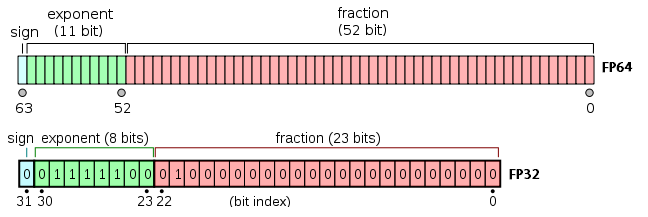
\includegraphics[width=\textwidth]{images/Floating_Point_structure.png}
		\caption {Структура чисел с плавающей точкой}
	\end{figure}
	
\end{frame}

\begin{frame}{Характериситки видеокарты}{Бенчмарки (benchmark)} 
	\begin{figure} 
		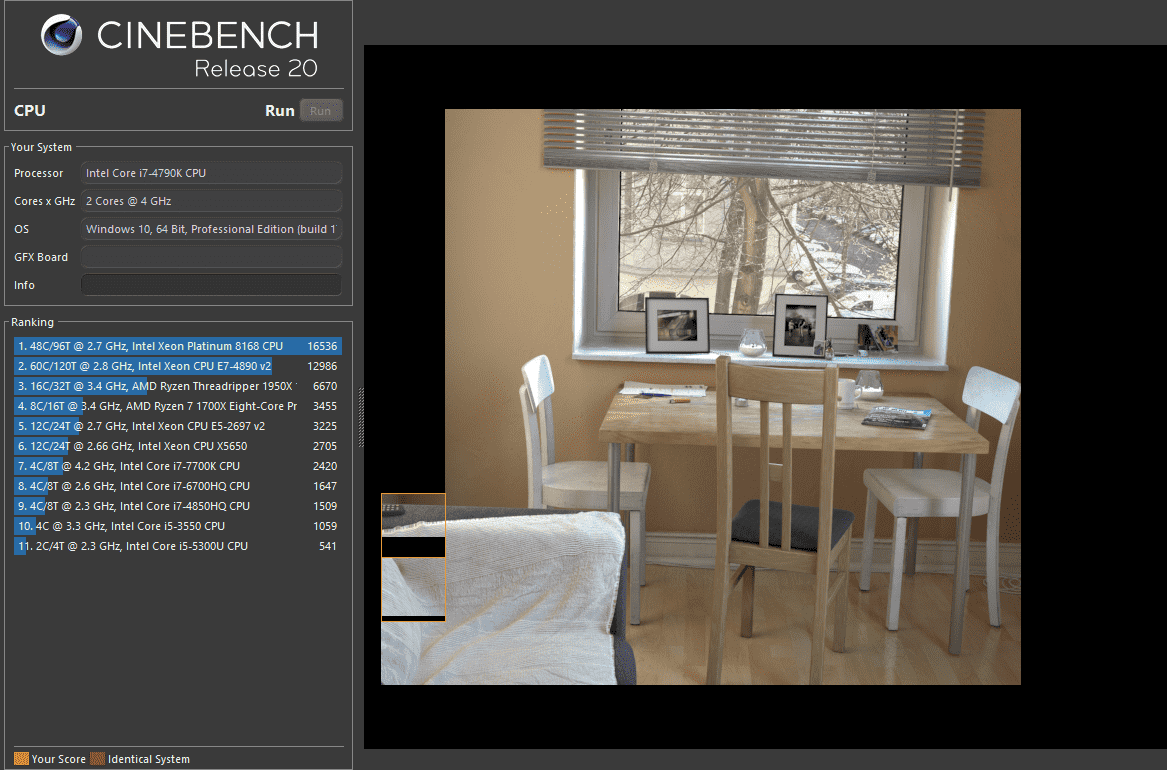
\includegraphics[width=0.8\textwidth]{images/Cinebench.png}
		\caption {Cinebench R23}
	\end{figure}
	
	\note{
		https://youtu.be/-bab7HjoZqk?si=HF1GxvNNv3mtCaRG
	
	Популярные
		\begin{itemize}
		\item 
		Cinebench R23
		\item 
		Furmark
		\item 
		3DMark
		\item 
		Heaven
		
	\end{itemize}
	
	и др.
	}

\end{frame}

\section{Программные средства}
\begin{frame}{Терминология}
	{\scriptsize
	
	\textbf{Спецификация (стандарт)} --- документированные наборы правил, рекомендаций и параметров, определяющие способы взаимодействия, описание, единое понимание и совместимость между аппаратной и программной частями.
	
	\textbf{Драйвер (видеодрайвер)} --- программный интерфейс между операционной системой и графическим аппаратным обеспечением компьютера или устройства. 
	%Графический драйвер выполняет важную роль в управлении и координации графическими функциями, такими как отображение изображений, обработка графики и управление монитором. Он обеспечивает абстракцию между аппаратурой и приложениями, позволяя программам использовать графические возможности устройства без необходимости знания специфических деталей аппаратной реализации.
	
	\textbf{Графическая библиотека} --- набор программных инструментов, функций и ресурсов, предназначенных для упрощения создания графических элементов в компьютерных приложениях. 
	%Графические библиотеки предоставляют разработчикам доступ к базовым операциям рисования, управлению окнами, обработке ввода и другим визуальным компонентам.
	
	\textbf{Графический движок} --- программное обеспечение, которое предоставляет инфраструктуру и инструменты для разработки интерактивных графических приложений, игр и визуальных симуляций. 
	%Графические движки обычно включают в себя готовые решения для управления графикой, физикой, анимацией, освещением и другими аспектами визуализации.
	
	\textbf{Графический фреймворк} --- комплексная структура, предоставляющая базовую архитектуру и инструменты для разработки графических приложений. 
	%В отличие от графических библиотек, фреймворки предоставляют более высокоуровневую абстракцию, объединяя не только графические, но и другие компоненты, такие как управление событиями, многозадачность и др.
	
	\textbf{Графические редакторы} --- программное обеспечение, предназначенное для создания, редактирования и манипулирования графическими изображениями, включая различные эффекты, анимацию и многое другое. 
	%Графические редакторы могут быть ориентированы на векторную или растровую графику, обеспечивая пользователю инструменты для рисования, изменения цветов, добавления эффектов и других операций над изображением.
	
	\textbf{Графический профилировщик} --- программное обеспечение, используемое для анализа и оптимизации производительности графических приложений или систем. 
	%Графический профилировщик собирает данные о времени выполнения, использовании ресурсов (например, CPU и GPU), вызовах функций и других аспектах работы с графикой. Эти данные помогают разработчикам и инженерам идентифицировать узкие места, проблемы с производительностью и оптимизировать код или конфигурацию, чтобы обеспечить более плавное и эффективное взаимодействие графических приложений с аппаратурой и операционной системой.
	
	\textbf{GPU benchmark (бенчмарк графического процессора)} --- методика тестирования и оценки производительности графического процессора, которая позволяет измерить его способность обрабатывать графику и выполнение вычислительных задач. 
	%В ходе GPU бенчмарка используются специально разработанные тестовые сцены или наборы задач, которые загружают графический процессор различными видами нагрузки, включая визуализацию 3D-графики, обработку текстур, вычисления с плавающей точкой и другие графические задачи. Результаты бенчмарка позволяют оценить производительность GPU, сравнить его с другими моделями или системами, а также определить, какие виды задач выполняются наиболее эффективно, что может быть полезно при выборе аппаратного обеспечения для конкретных целей.
}
\end{frame}


\begin{frame}{Графические библиотеки и спецификации}{Программный интерфейс (или API, Application Programming Interface)}
	{\small
	\textbf{OpenGL (1992, Silicon Graphics)} \\
	Открытая кросс-платформенная спецификация для работы с 2D и 3D графикой
	
	\textbf{Mesa (1995)} \\
	Свободная реализация графических API OpenGL (позже Vulkan и др.) с открытым исходным кодом
	
	\textbf{DirectX (1995, Microsoft)} \\
	Пакет графических API для работы с играми и мультимедийными приложениями на платформе Windows
	
	\textbf{WebGL (2011,	Khronos Group)} \\
	Графический API для веб-браузеров 
	
	\textbf{Mantle (2013, AMD)} \\
	Спецификация низкоуровневого API
	
	\textbf{Vulkan (2016, Khronos Group)} \\
	Низкоуровневый высокопроизводительный кроссплатформенный API для работы с 2D и 3D графикой
	}
	\if 0
	
	1992 OpenGL (Open Graphics Library) 	Khronos Group 
	Открытая кросс-платформенная спецификация для работы с 2D и 3D графикой
	
	1991	Qt	The Qt Company	Кроссплатформенный фреймворк и GUI
	1995	OpenGL	Khronos Group	Открытый стандартный API для 2D и 3D графики
	2000	SDL	Sam Lantinga	Простая библиотека для работы с мультимедиа
	2001	DirectX	Microsoft	Набор API для разработки игр на Windows
	2005	Unity	Unity Technologies	Интегрированная среда разработки игр
	2007	SFML	Laurent Gomila	Простая и понятная библиотека для C++
	2011	Vulkan	Khronos Group	Высокопроизводительный API для графики
	2012	WebGL	Khronos Group	Графический API для веб-браузеров
	
	
	1991	OpenGL	Khronos Group	Кросс-платформенная библиотека для работы с 2D и 3D графикой, открытый стандарт
	1995	DirectX	Microsoft	Пакет графических API для работы с играми и мультимедийными приложениями на платформе Windows
	2001	Qt	The Qt Company	Кросс-платформенный фреймворк для создания графических приложений с широким набором функциональности и инструментов
	2003	SDL	Sam Lantinga, others	Простая кросс-платформенная библиотека для работы с графикой, звуком и вводом в играх
	2007	Unity	Unity Technologies	Интегрированная среда разработки для создания 2D и 3D игр, поддерживает различные платформы и имеет обширный магазин активов
	2010	Vulkan	Khronos Group	Низкоуровневый открытый стандарт для работы с графикой, обеспечивающий бо
	
	\fi
	
	
\end{frame}


\begin{frame}{Структура графической библиотеки}
	\textbf{Графический движок} (движок рендеринга 2-х или 3-х мерной КГ)
	
	%Порядок приоритетов поменять
	
	\begin{itemize}
		\item 
		Должны работать в реальном времени
		\item 
		Поддержка шейдеров
	\end{itemize}
	
	\textbf{Анимация}
	\begin{itemize}
		\item 
		Кинематика(компьютерный фильм)
	\end{itemize}
	
	\textbf{Физический движок }(физика)
	\begin{itemize}
		\item 
		Динамика жидкости, газа, взаимодействия тел и т.д.
	\end{itemize}

	\textbf{Игровой ИИ} (game artificial intelligence)
	\begin{itemize}
		\item 
		Боты (bots), моды (mods) и неигровые персонажи (non-player characters)
	\end{itemize}
	
	\textbf{Звук, система скриптов (система I/O), сетевой интерфейс} и т.д.
\end{frame}

\begin{frame}{Распределение вычислений между CPU и GPU}{Central and Graphical Processor Unit}
	%GPU а термин не ввел.
	\begin{figure} 
		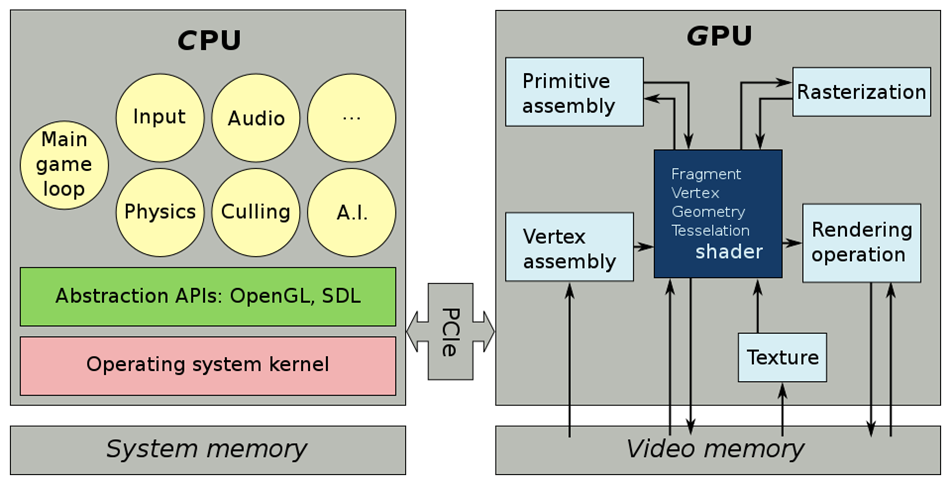
\includegraphics[width=0.95\textwidth]{images/Calculation_distribution_scheme.png}
		\caption {Принципиальная схема распределения вычислений}
	\end{figure}
\end{frame}

\begin{frame}{Конвейер рисования в OpenGL}{}
	\begin{figure} 
		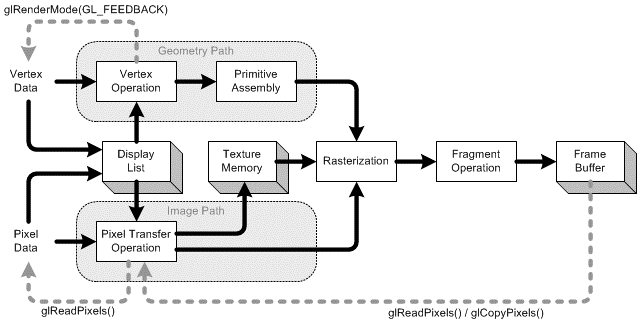
\includegraphics[width=0.95\textwidth]{images/OpenGL_graphics_pipeline.png}
		\caption {Принципиальная схема распределения вычислений}
	\end{figure}
\end{frame}


\begin{frame}{Упрощенная модель графического конвейера}{Shaders}
	\begin{columns}
		\begin{column}{0.5\textwidth}
			\begin{figure} 
				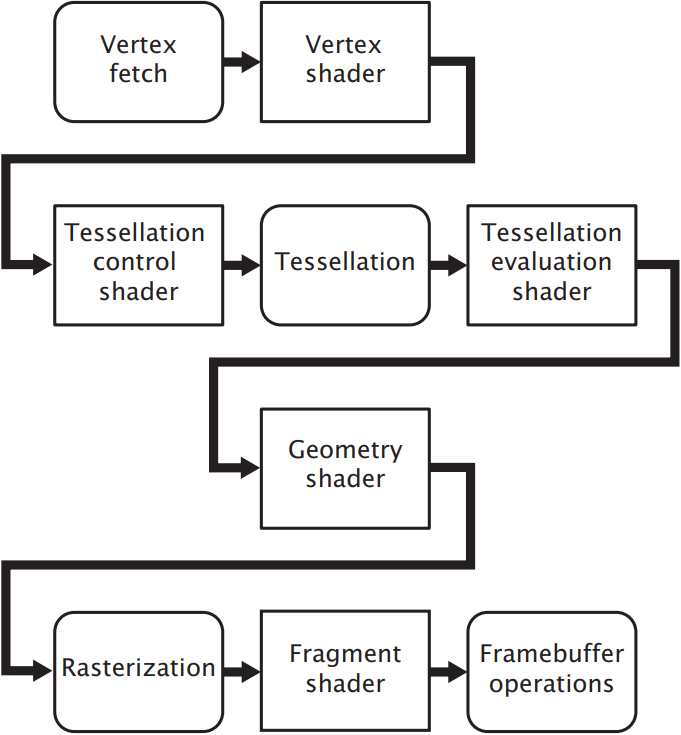
\includegraphics[width=0.9\textwidth]{images/Simplified_model_of_the_graphics_pipeline.png}
				\caption {Порядок вычисления шейдеров}
			\end{figure}
		\end{column}
		\begin{column}{0.5\textwidth}
			
			{\footnotesize
			
			Загрузка данных
			
			{\hfill Вершина (vertices)}
			
			\textbf{Вершинный шейдер}
			
			{\hfill Группа вершин (primitives/patches)}
			
			\textbf{Шейдер управление тесселяцией}
			
			Тесселяция
			
			\textbf{Шейдер определяющий тесселяции}
			
			{\hfill Примитивы (primitives)}
			
			\textbf{Геометрический шейдер}
			
			{\hfill Примитивы (primitives)}
			
			Растеризация и интерполяция
			
			{\hfill Пиксели (fragments)}
			
			\textbf{Пиксельный (фрагментный) шейдер}
			
			{\hfill Пиксели (fragments)}
			
			Операции с буферами кадров
			
			{\hfill Пиксели (Pixels)}
		}
		\end{column}
	\end{columns}
	

\end{frame}


\begin{frame}{Упрощенная модель графического конвейера}{OpenGL specification}
	\begin{figure} 
		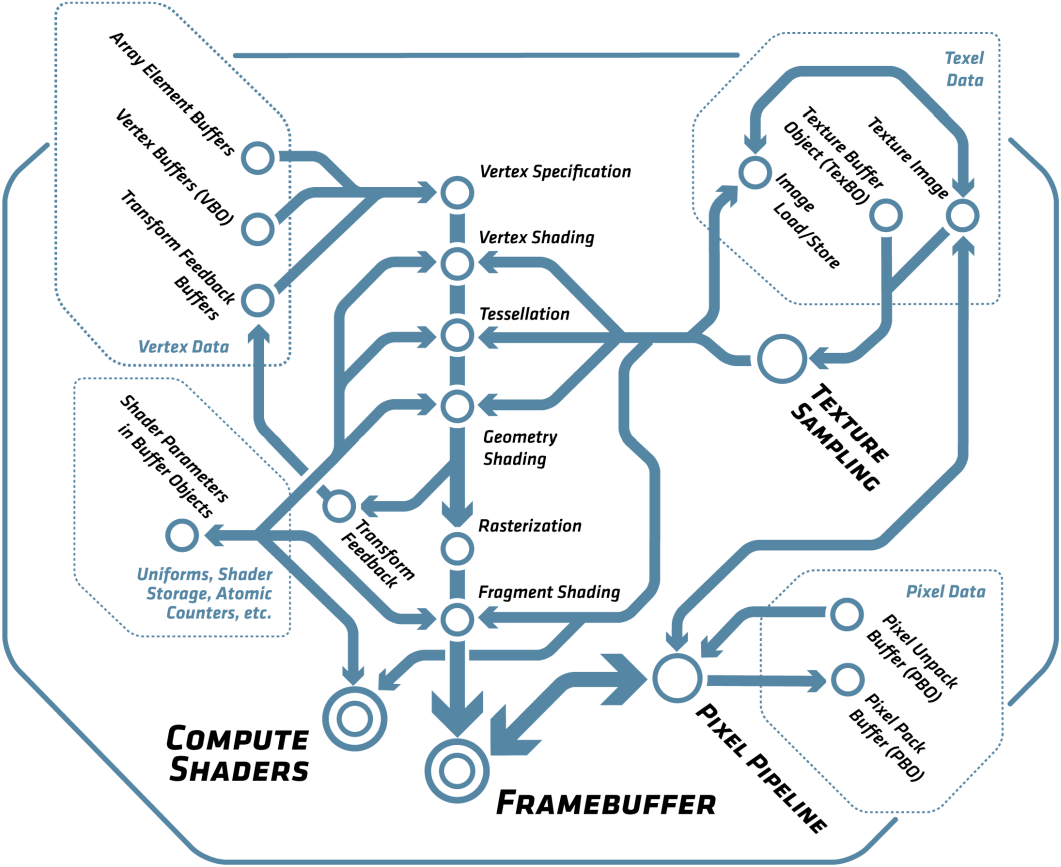
\includegraphics[width=0.65\textwidth]{images/OpenGL_specification_graphics_pipeline.png}
		\caption {Принципиальная схема распределения вычислений}
	\end{figure}
\end{frame}

\if 0
\begin{columns}
	
	\begin{column}{0.5\textwidth}
		\begin{itemize}
			\item
			
		\end{itemize}
	\end{column}
	\begin{column}{0.5\textwidth}
		\begin{itemize}
			\item
		\end{itemize}
	\end{column}
	
\end{columns}
\fi
	
\end{document}